\chapter{DNA sequence classification} \label{sec:dna_sequences}

\section{DNA sequences} \label{subsec:what_are_dna_sequences}

\gls{DNA} is composed of a linear string of nucleotides, or bases, which are referred to by their chemical names' first letters: \gls{A}, \gls{T}, \gls{C}, and \gls{G}. 

\gls{DNA} sequencing is the technique of finding the order of the four bases. Scientists can determine the type of genetic information carried in a \gls{DNA} segment by examining the sequence. Furthermore, and more significantly, sequencing data can reveal mutations in a gene that could lead to illness, by comparing a healthy and a mutated sequence~\cite{2020DNASheet}.

The four chemical bases of the \gls{DNA} double helix always connect with the same partner to produce "base pairs". \gls{A} is always paired with \gls{T}, while \gls{C} is always paired with \gls{G} (Figure~\ref{fig:dna}). This pairing explains the technique by which \gls{DNA} molecules are copied when cells divide, as well as the methods used in most \gls{DNA} sequencing research. The human \gls{genome} is made up of around 3 billion base pairs, which carry the instructions for creating and maintaining a human person~\cite{2020DNASheet}.

\begin{figure}[htbp]
    \centering
    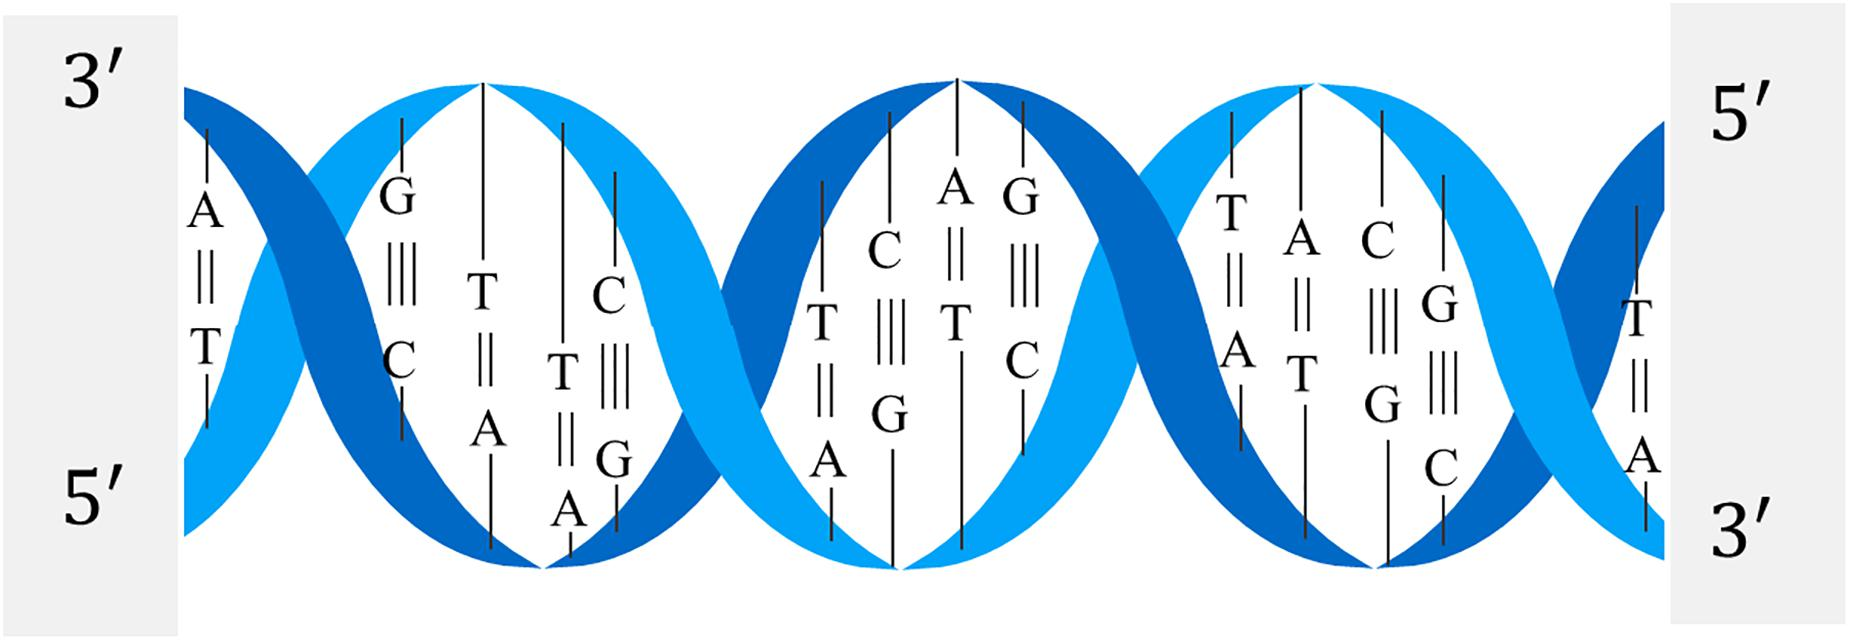
\includegraphics[width=0.5\linewidth]{Chapters/Figures/dna.jpg}
    \caption{Double helix of DNA~\cite{Yang2020ReviewDNA}}
    \label{fig:dna}
\end{figure}

Since the Human Genome Project's completition~\cite{TheProject}, technological advancements and automation have made it possible for individual genes to be sequenced on a regular basis, by reducing the amount of time it takes to perform the sequencing and also reducing its cost. Some labs can sequence over 100,000 billion bases per year, and a few thousand dollars is enough to sequence an entire \gls{genome}~\cite{2020DNASheet}. 

\section{DNA sequence classification - Traditional ML}

With the rapid development of sequencing technology in the post-genomic era, the amount of biological sequence data (\gls{DNA}, \gls{RNA}, and protein sequences) is rapidly increasing. However, structural and functional data from wet-lab investigations are still limited due to the time and cost of the research. The difference between sequence and structural data is rapidly widening. These sequences are essential for basic research (studying the structure and function of \gls{DNA}, \gls{RNA}, and proteins) as well as applications (disease research, precision medicine, etc.). Many effective and computationally affordable approaches for analyzing sequence data have recently been presented. Because the majority of sequence analysis tasks may be expressed as binary classification or multiclass classification tasks, \gls{ML} techniques play an important role in these challenges~\cite{Liu2019BioSeq-Analysis:Approaches}.

In \gls{ML}, classification is an essential mining task. Its goal is to use the training sample set to create a classification model that can predict the category of unknown incoming samples. \gls{DNA} sequence classification is the process of predicting the kind of \gls{DNA} sequence based on structural or functional similarities, then predicting the sequence function and relationships with other sequences, and finally assisting in the identification of genes in \gls{DNA} molecules~\cite{Yang2020ReviewDNA}.

It is worth emphasizing that feature extraction is especially important for sequence analysis. Converting sequences into an effective mathematical expression that genuinely reflects the underlying relationship with the feature to be predicted can have a big impact on the model's performance~\cite{Chen2020ILearn:Data}.

It is standard practice to encode molecular information as numerical features in order to apply various \gls{ML} algorithms to molecular data. The kind of encoding has a significant impact on studies, therefore picking an accurate and effective encoding is crucial. Molecular descriptors are one of the most powerful tools for describing the biological, physical, and chemical features of molecules, and they have been utilized in a variety of research to better understand molecular interactions and drug development for a long time. These descriptors capture and amplify different features of molecular topology in order to better understand how molecular structure influences molecular properties~\cite{Dong2018PyBioMed:Interactions}. Tools such as
\textit{BioSeq-Analysis}~\cite{Liu2019BioSeq-Analysis:Approaches} and \textit{iLearn}~\cite{Chen2020ILearn:Data} are platforms capable of calculating descriptors for not only \gls{DNA} but also \gls{RNA} and protein sequences. In addition, these packages also perform \gls{ML} functions on the calculated features. \textit{BioSeq-Analysis} focuses on automatically completing the three main steps of \gls{ML} predictors, which are feature extraction, predictor construction, and performance evaluation.
\textit{iLearn} has functions for feature extraction, clustering, feature selection, dimensionality reduction, and ensemble learning, making it a more comprehensive package.

%Descriptors 
%Algorithms  

\section{DNA sequence classification - DL}

A common difficulty in data mining is classifying biological sequences as a specific data type. This is a tough challenge, due to the non-numerical properties of biological sequence elements, the sequence interaction between sequence elements, and the variable sequence length~\cite{Yang2020ReviewDNA}. This means that the feature selection method remains the most difficult aspect of the challenge. Sequences lack specific features, and the most often used representations add to the problem of excessive dimensionality. \gls{ML} methods for supervised classification tasks are, without a doubt, heavily reliant on the feature extraction stage, and it is required to detect and quantify relevant aspects of the objects to classify in order to develop a suitable representation. \gls{DL} models have recently been shown to be capable of automatically extracting meaningful features from input patterns~\cite{LoBosco2017DeepClassification}.

% (over strings?)
% common architectures